\documentclass[11pt,letterpaper]{article}
\usepackage[english]{babel}
\usepackage[utf8]{inputenc}
\usepackage{fancyhdr}
\usepackage[margin=1in]{geometry}
\usepackage{enumitem}
\usepackage{amsmath}
\usepackage{graphicx}
\usepackage{setspace} 
\usepackage{pdfpages}
\usepackage{xcolor}
\onehalfspacing
 
\pagestyle{fancy}
\fancyhf{}
\lhead{CS\&SS 569 HW 3}
\rhead{Nan Tang (1662478)}
\rfoot{Page \thepage}
 

\title{CS\&SS 569 Homework 3}
\author{Nan Tang 1662478}
\date{\today}
 
\begin{document}
\maketitle 

\subsection*{Data Description} 
\noindent This interactive display is based on the data of '2018 INDEX OF ECONOMIC FREEDOM', world’s premier measurement of economic freedom, ranking countries based on five areas: size of government, legal structure and security of property rights, access to sound money, freedom to trade internationally, and regulation of credit, labor and business. 

\subsection*{Purpose and Methods}

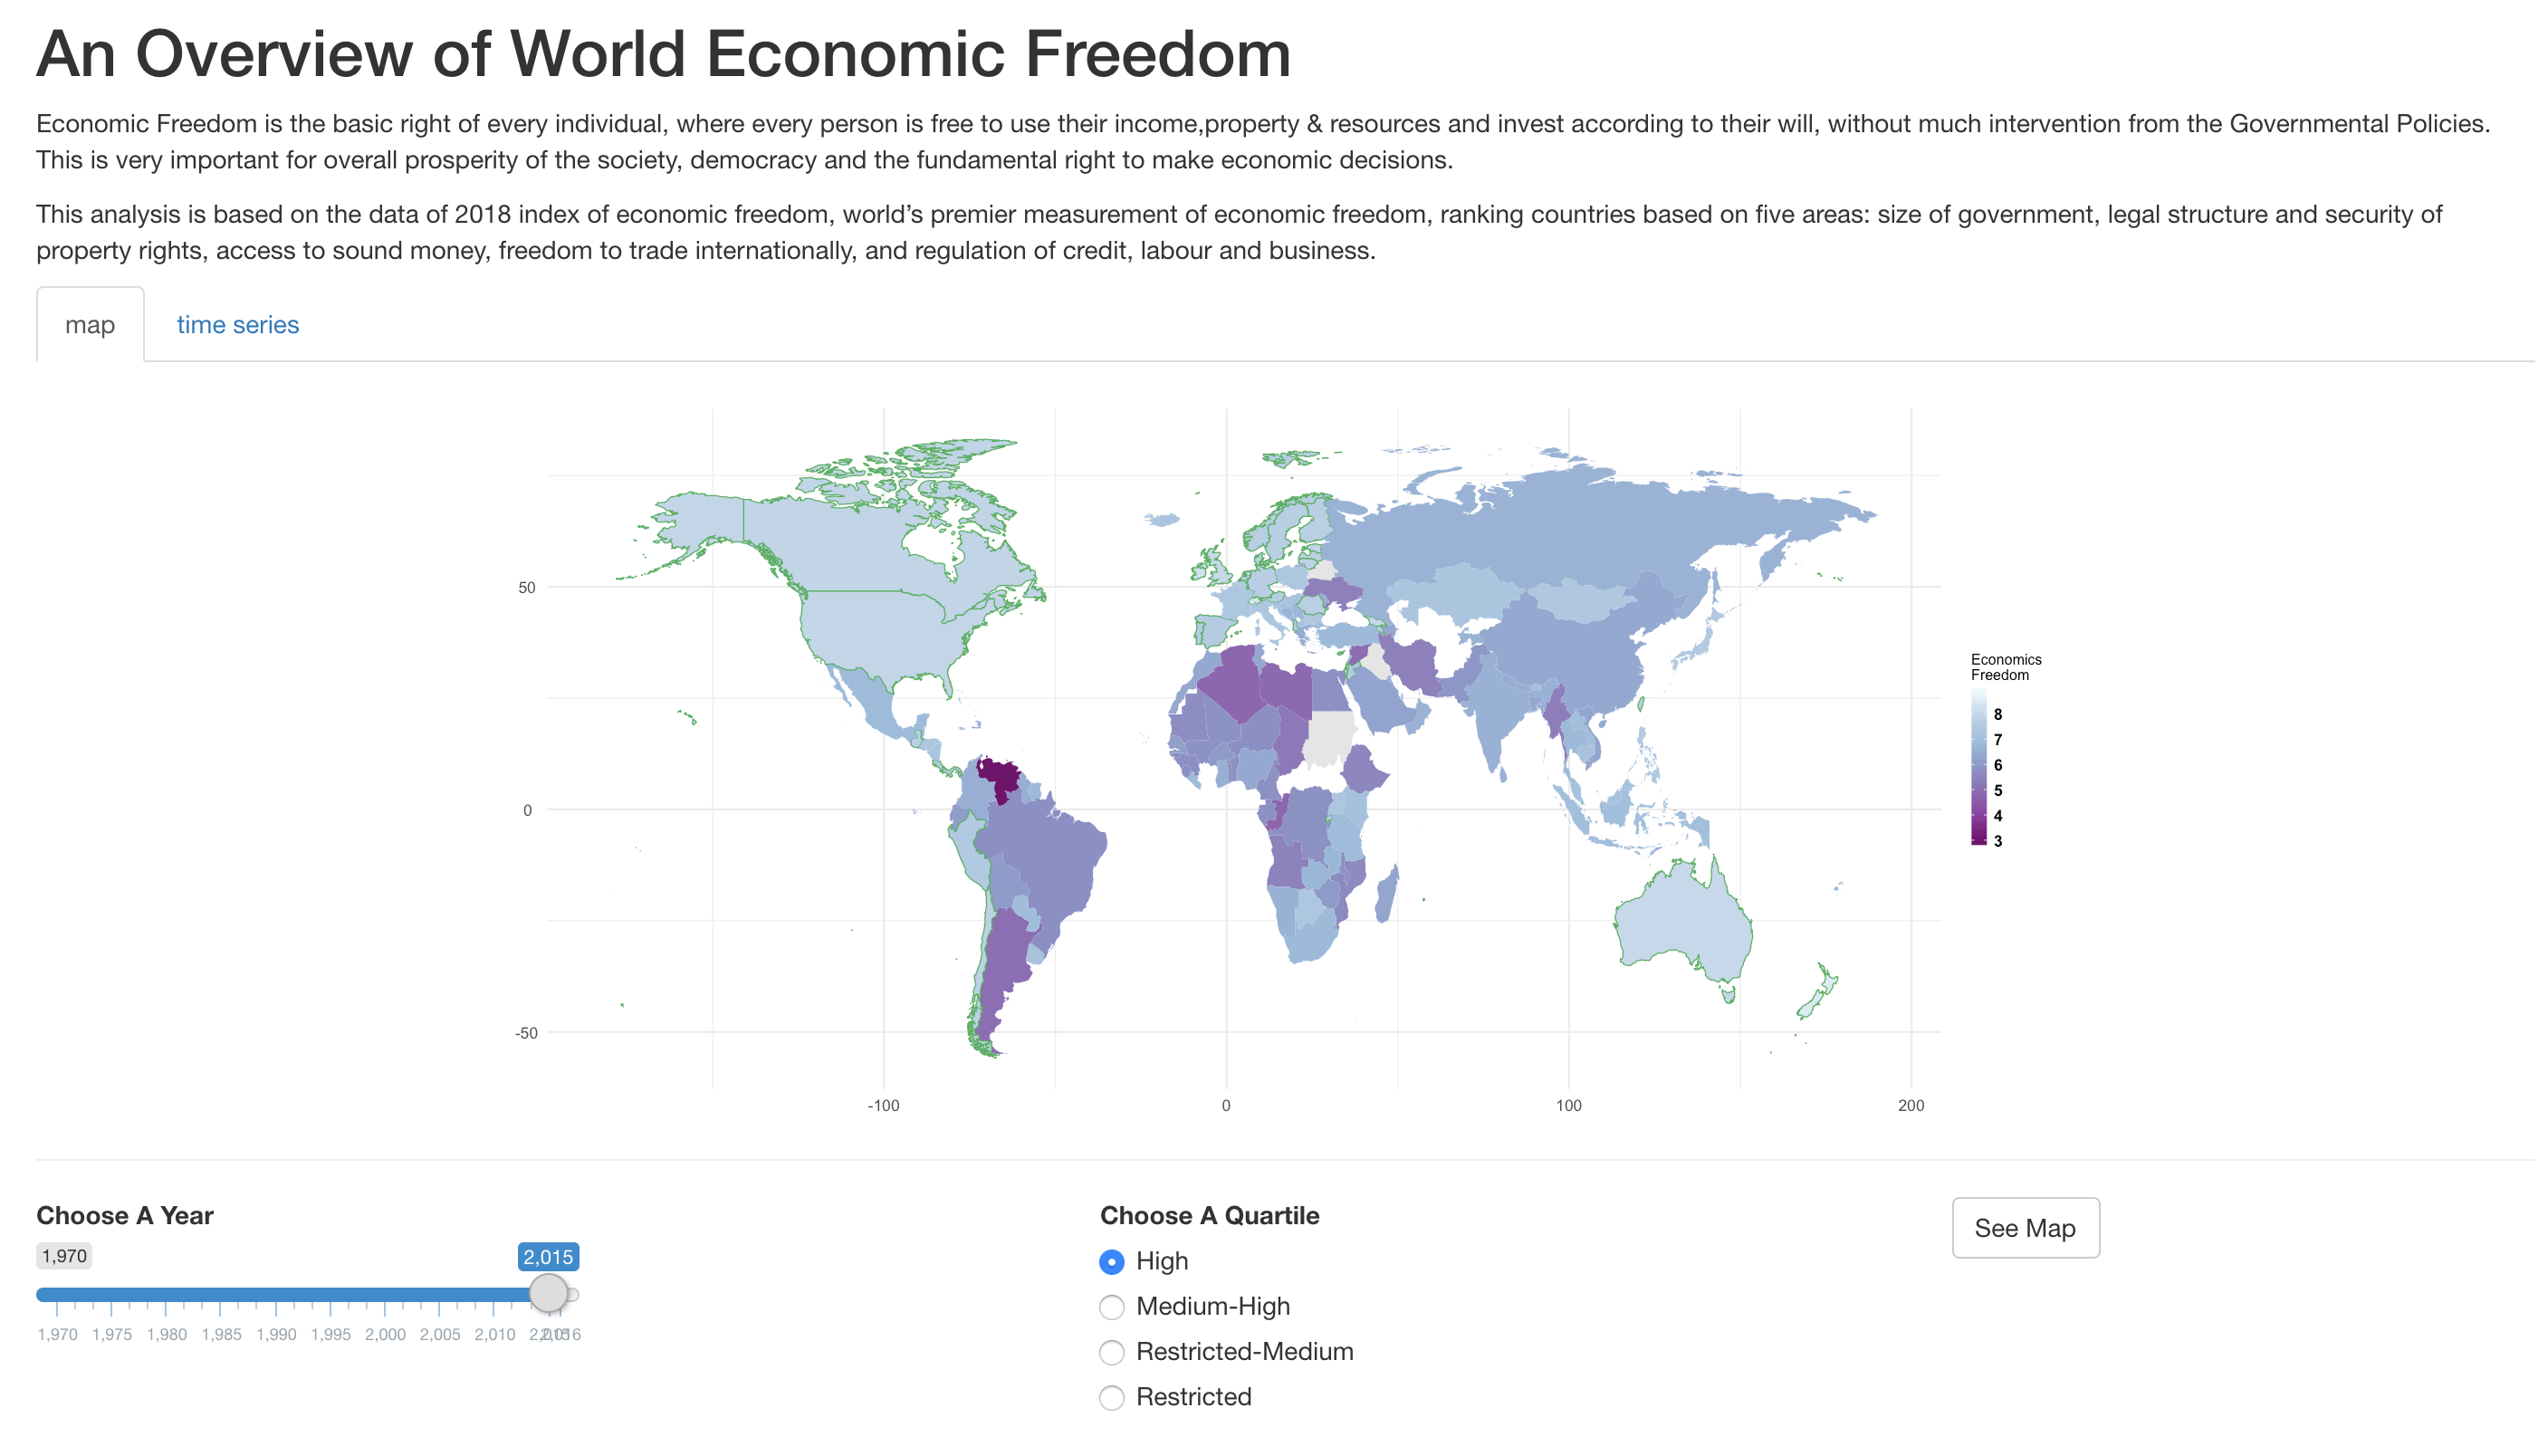
\includegraphics[width=6.5in]{hw3-1.png} 

\noindent Interactive visual is a great method to provide users with holistic view on multidimensional data or events. It is especially suitable for the world economic freedom, which extends to both dimensions of time and space. This interactive visual display is consist of two tabs. The first part shows the economic freedom index (ranking) for all countries in chosen year. Countries in dark purple generally have more restrictions on economic activities than countries in bright purple. Users are free to choose a year of interest from the scrolling bar. Beside the scrolling bar, I set another check box for quartile of the countries. Countries within the chosen quartile are enclosed with green border, so that users who are less sensitive to color intensity could easily check the quartile of countries they are interested in. The purpose of first tab is to generate the spatial pattern of world economic freedom. Spacial pattern is not enough. In order to provide a holistic view of the dataset, I set up the second tab for time series data. \\

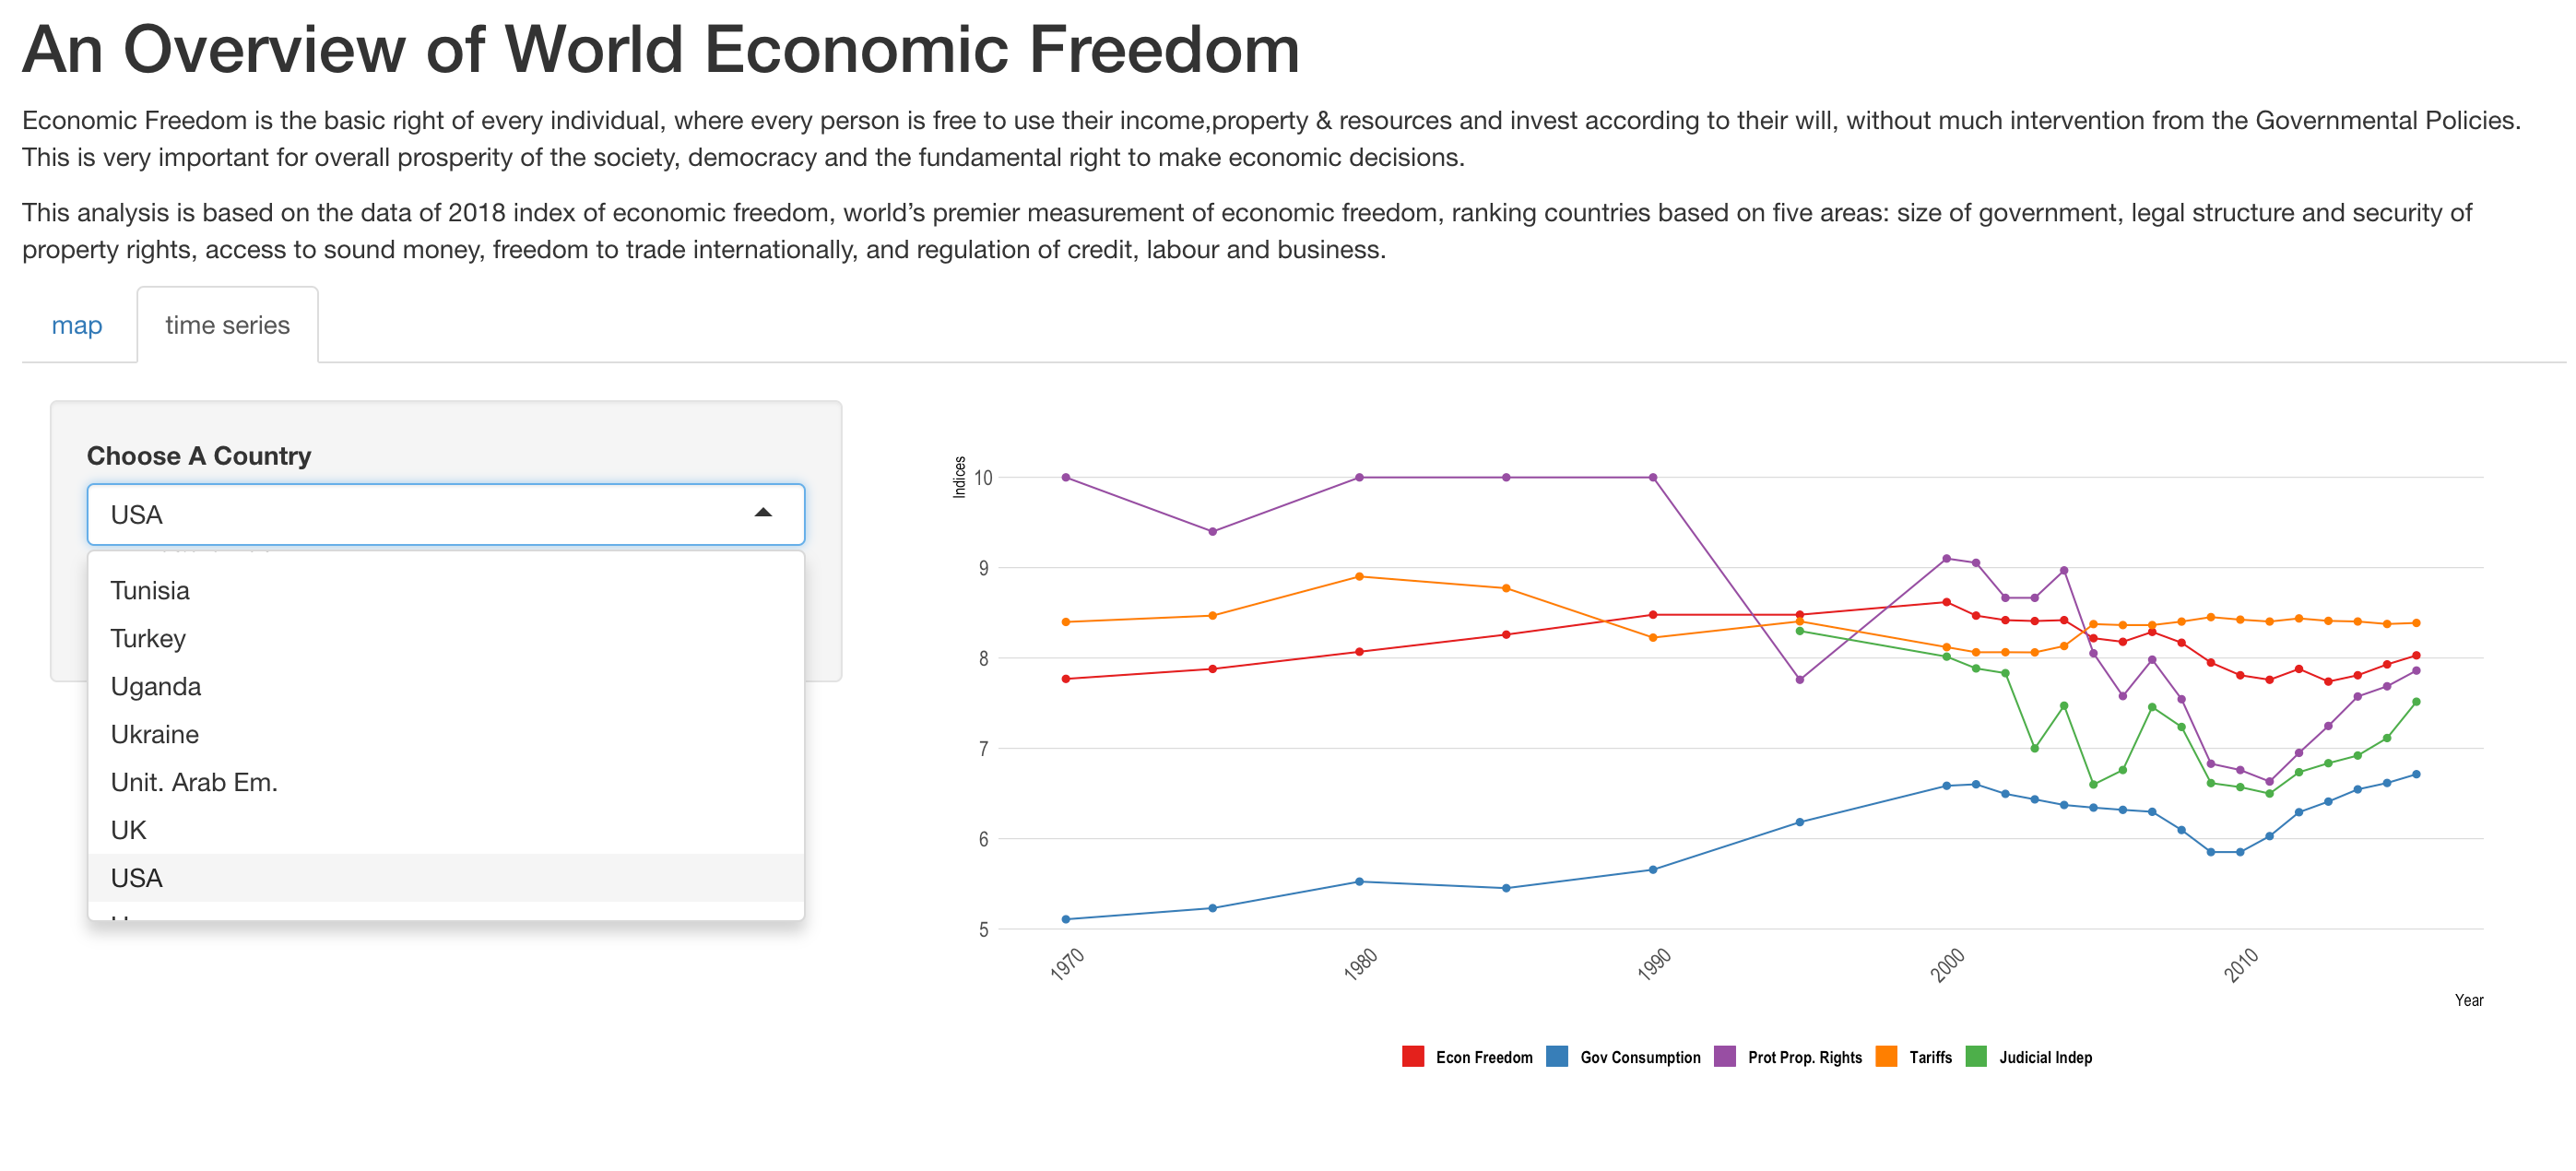
\includegraphics[width=6.5in]{hw3-2.png} 

\noindent On this tab, users could check time series data for any chosen country. Base on previous research, I picked four other indices, government consumption, protection of property right, tariff, and judicial independence, that are significantly related to result of economic freedom. For the US, the trend of economic freedom and other variables are not very obvious, however, for developing countries such as Russia and China, users could perceive the significant effectiveness of four other indices on the economic freedom index from time-related trend. 
 
 
 
\end{document}